\section{Toward web3}
During the evolution of internet we had:
\begin{itemize}
    \item Internet: just a bunch of wires and interconnected network;
    \item Web 1.0: read-only and static, everyone can add stuff but no interaction is possible;
    \item Web 2.0: read-write but interactive, everyone can add stuff to the network and even interact with them;
    \item Web 3.0: read-write-trust and even verifiable: exploit cryptographic primitives and distribution.
\end{itemize}

IPFS is a p2p protocol making the web upgradeable , resilient and opened and can be seen as a p2p content-based version of HTTP.
It was created by Protocol Labs which is an open source R\&D lab which builds protocols, tools and service to improve Internet.
They developed Filecoin too which is a decentralized storage network to store web's content.

The main idea behind IPFS is to avoid the use of centralized server for some services in order to:
\begin{itemize}
    \item fight censorship: if data is distributed you can't block the server who is distributing content;
    \item improve bandwidth utilization: by spreading content around the Internet it is easier to get them from nearer peer;
    \item make web more open.
\end{itemize}

In IPFS you address the content instead of the container, because you don't care who is actually hosting the content, all you care is the content.

IPFS combines:
\begin{itemize}
    \item a distributed hashtable;
    \item an incentivized block exchange (it's not blockchain!);
    \item a self-certifying namespace.
\end{itemize}
In particular it leverages many successful p2p system ideas:
\begin{itemize}
    \item routing: DHT with a set of improvement for security (S/Kademlia) and performance (sloppy hierarchical DHT);
    \item block exchangers: BitTorrent;
    \item version control systems: Git;
    \item Self-Certified FileSystems: SFS.
\end{itemize}

\section{IPFS}
\subsection{Key ideas}
The idea is to build a global distributed file system: IPFS is about \emph{distribution of control} with content-based identification with secure hash of contents through DHT.
The blocks are exchanged using Bittorrent-like protocol incentivizing block exchange using Bitswap protocol.
Files are organized with Merkle DAG (the same as merkle tree but with blocks that represents a directory-file structure) and are version-based, similar to Git for instance.
Using that data structure one can build versioned file systems, blockchains, and so on.
For security reasons self-certification servers are used for the storage nodes.

\subsection{In a nutshell}
Adding a photo to IPFS it's is converted in raw data and in order to make it content addressable it is hashed obtaining a unique \emph{digest}.
Using cryptographic hashes we inherit some properties:
\begin{itemize}
    \item tamper-freeness: if we change even a single pixel in the input, the output will be completely different;
    \item verifyability via self-certifying file systems you can transfer the image to anybody, he/she can check that the photo received has not been tampered;
    \item security: you cannot tell which is the input just seeing its output.
\end{itemize}

The hash as it is is then transformed to a CID (Content Identifier) which is the real identifier of the content, used to address it in the network.
Since we are using the hash to do it the content is inherently immutable because any change updates the content, changes the hash and so the CID.
To solve this problem older version of the content can be referenced through IPNS.
Moreover the CID contains several metadata like the \emph{multihash}: the hash value alongside with a descriptor of the hashing function employed and the size.
This allows multiple hash functions to co-exists, this way if one the hash turns out to be broken the entire system does not need to change, cause there are several.

Large files are broken into chunks equal or smaller than 256k, a CID is produced for each chunk and then they are combined to create the base CID using a Merkle CID.

In order to download the content we need to locate the resource, IPFS exploit a DHT to map CID to peers addresses that have the content.

\subsection{IPLD}
IPFS uses IPLD (Interplanetary Linked Data) for managing complex objects and it's based on the idea of linked data for decentralizing the web.
IPLD exploits Merkle DAGs for managing all the chunks and linking them to the base CID.

The IPFS Object contains both data, up to 256kb, and a set of links.
Each IPDL link has 3 parts:
\begin{itemize}
    \item name;
    \item hash of the linked Object;
    \item cumulative, recursive size of the IPFS object.
\end{itemize}
Using those IPFS Objects we can build a full file system.

The linked data has the advantage of deduplication: the same content is stored only once because two identical stuff will have the same identical hash and so the peer can store only one, saving storage.

\subsection{IPNS}
The hash link to content in IPFS are not human readable and immutable, to avoid that everytime a resource changes you have to share again the CID IPNS was invented.
IPNS (Interplanetary Naming System) is a system allowing to always point to the latest version of a content, it can be human readable and easy to remember, something like DNS for IPFS.

\subsection{IPFS stack}
\begin{figure}[H]
    \centering
    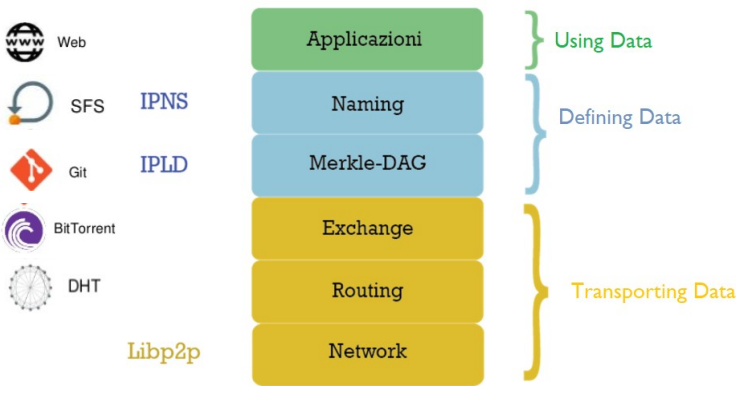
\includegraphics[width=300px]{images/11_IPFS/01.png}
    \caption{IPFS stack}
\end{figure}

\subsubsection{Exchange level}
Bitswap is a protocol for data exchange (in our case block exchange): files are split into blocks, the smallest unit of transferable data, inspired to the principles of BitTorrent but with some differences: Bittorrent allows a separate swarm of peers for each file while IPFS allows only a single swarm of peers for all the data shared by the users.

The whitepaper of the protocol describes a basic bartering strategy for block exchanges and above this a virtual currency can be defined, for example Filecoin.

\subsubsection{Routing level}
IPFS uses the hash of the file as a key to return the location of the file, once the location is determined, the transfer takes place peer-to-peer as a decentralized transfer.
In order to make DHT really works IPFS takes ideas from S/Kademlia and Coral Sloppy DHT.

S/Kademlia is a secure key-based routing protocol based on Kademlia, it's high resilience against common attacks and offers a set o fsecurity improvement with respect to Kademlia like:
\begin{itemize}
    \item limitation of free node identifier generation: it uses PoW and public key cryptography to verify messages;
    \item parallel look-ups over multiple disjoint paths;
    \item extension of Kademlia routing table by a sibling list.
\end{itemize}

\subsection{File availability}
Each node of the network keeps a cache of the files it has both downloaded or shared, those info will be shared if other people needs them, like a Bittorrent swarm but with a single swarm for all the elements, instead of one for each content.

However if all nodes owning a file go offline the file becomes unavailable.
The protocol needs to incentivize nodes to store files and make them available or to proactively distribute files trying to guarantee a number of copies in the network.

\subsection{Versioning}
IPFS supports versioning of files so when a file is modified the new version is registered and old versions are maintained.
It keeps all the story of the web content making data immutable.

Basically IPFS builds commits with a parent pointer to previous commit.

\section{Filecoin}
Filecoins (FIL) is a cryptocurrency built over IPFS to build a decentralized market for storage.
If you have free space on disk you can make money storing files of other users.

It's a decentralised alternative to Google Drive and Dropbox, also the hyper-competitive market means the prices for storage are fairer compared to those offered by centralized alternatives, moreover in Filecoin, all the storage in the world that isn't being used can be put to use, instead of making new storage.

FIL token is used by clients to pay for storage on the network, and also as reward for miners to executing tasks like storing data, securing the network and paying trancation fees.

\section{Multiformat project}
It's a collection of standards and protocols suitable to support future software modifications.
The project began with IPFS and now it is used also for other projects.

It could be useful for example because current hash function may be broken and hard-wiring such algorithms in the code implies modifying lots of codebases when it will happen.

This project points to enhance data format values with self-descriptions:
\begin{itemize}
    \item together the value itself;
    \item as small as possible;
    \item no lock in;
    \item interoperability;
    \item agility.
\end{itemize}

Nowadays some protocols have already been developed:
\begin{itemize}
    \item multihash: self-describing hashes;
    \item multiaddr: self-describing network addresses;
    \item multibase: self-describing base encodings;
    \item multicodec: self-describing serialization;
    \item multigram: self-describing packet network protocols.
\end{itemize}

\subsection{Multihash}
It's a self describing hash which includes the hash value with a prefix.
It uses the TLV pattern: type-length-value in which the type identifies the cryptographic algorithm according to a multicodec table.
A multicodec table contains codes for:
\begin{itemize}
    \item hash functions;
    \item serialization functions (JSON, protobuf, ...);
    \item internet protocols;
    \item ...
\end{itemize}


\section{libp2p}
It's a p2p network stack introduced by the IPFS community.
It was born as a subproject of IPFS but used by many other projects.

It allows to:
\begin{itemize}
    \item peer identity via public key cryptography;
    \item secure communications through ecrypted channels;
    \item peer routing using Kademlia;
    \item content discovery using Kademlia;
    \item generation of a key-pair to secure communication channels and of PeerId generated by hash of peer's public key.
\end{itemize}






